\documentclass{beamer}
%\documentclass[handout]{beamer}

\usepackage{pgfpages} 
%\pgfpagesuselayout{4 on 1}[letterpaper,border shrink=5mm,landscape] 
%\pgfpagesuselayout{2 on 1}[letterpaper,border shrink=2mm]

\setbeameroption{notes on second screen}

\usetheme{default}

\mode<presentation> {
%  \usetheme{Warsaw}
  \usetheme{Frankfurt}
%  \usetheme{Boadilla}
%  \usetheme{Marburg}
}

\mode<handout>{\setbeamercolor{background canvas}{bg=black!5} %
    \pgfpagesuselayout{2 on 1}[letterpaper,border shrink=4mm] }

\title[CAC Intro] {A Introduction to\\ Linux }
\author{Brock Palen\\ \texttt{brockp@umich.edu}}
\date{TBD}

\begin{document}
  \setbeamercovered{transparent}  
  \begin{frame}
    \titlepage
  \end{frame}

%table of contents
  \begin{frame}{Outline}
    \tableofcontents
  \end{frame}
  
  \section{Connecting}
  \subsection {Secure Shell}

  \begin{frame}{ssh}
    \begin{block}{ssh}
    \begin{itemize}
    \item \texttt{ssh} is a secure method to access remote systems
    \item A single user may have many \texttt{ssh} conections
    \item A single system may have many users
    \item Both data and authentication information is protected
    \item<2-|alert@1->Never use \texttt{telnet} even if available
    \end{itemize}
    \end{block}
  \end{frame}
%nyx
  \begin{frame}{ssh clients}
    \begin{block}{ssh clients}
    \begin{itemize}
    \item <1->Windows: CAEN \texttt{ssh} Clent: \\
\alert{fix this}
        Start$\rightarrow$Programs$\rightarrow$Communication Tools$\rightarrow$SSH Secure Shell
    \item <2->Windows: Putty, Available for free: \\
        \url{www.chiark.greenend.org.uk/~sgtatham/putty/}
    \item <3->Linux, Unix, Mac OS: Use native clients
    \end{itemize}
   \end{block}
  \end{frame}

%windows clients CAEN
  \begin{frame}{CAEN SSH Client}
    \begin{block}{CAEN SSH Client}
    \begin{itemize}
      \item click ``Quick Connect'': \\
    \end{itemize}
   \end{block}
      \begin{center}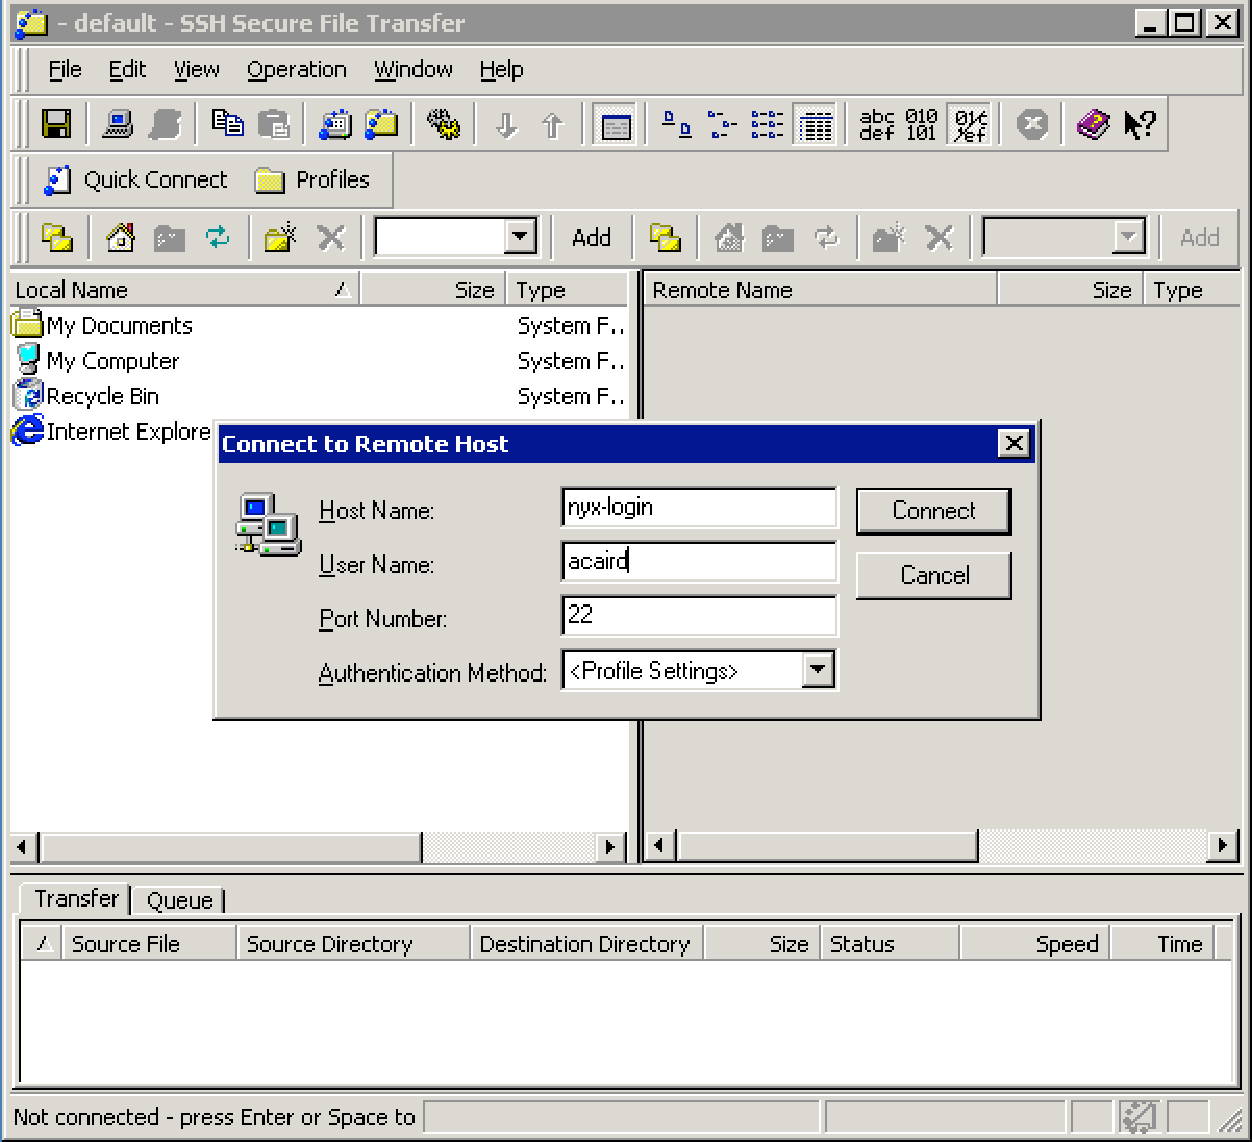
\includegraphics[width=2.5in]{ssh-sftp-login}\end{center}
  \end{frame}

%windows Client Putty
  \begin{frame}{Putty SSH Client}
    \begin{center}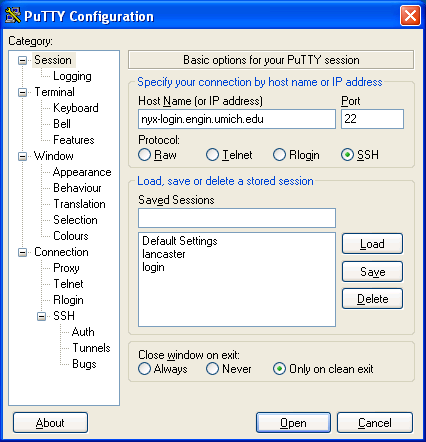
\includegraphics[height=2.25in]{ssh-putty-login}\end{center}
  \end{frame}
  
%SFTP
  \subsection {File Transfer}
  \begin{frame}{SFTP/SCP}
    \begin{block}{SFTP}
      Start$\rightarrow$Programs$\rightarrow$Communication Tools$\rightarrow$SSH Secure Shell
    \end{block}
    \begin{block}{SCP}
    \begin{itemize}
      \item Simple copy over SSH between two Unix/Linux hosts
      \item Send file: \texttt{scp localfile host:~/}
      \item Get file: \texttt{scp host:~/remotefile ~/}
    \end{itemize}
    \end{block}
  \end{frame}

%modules
\begin{frame}{Manipulating Software}
  All CAC systems use \texttt{modules} to control software. Users \textit{can} and \textit{should} write their own modules if needed.
  \begin{block}{module commands}
    \alert{make into table}
  \begin{itemize}
    \item \texttt{module list} \\ Show loaded modules
    \item \texttt{module load \textit{modulename}} \\  Load \textit{modulename} for use
    \item \texttt{module avail \textit{modulename}} \\ Show available versions of module \textit{modulename}
    \item \texttt{module rm \textit{modulename}} \\  Remove currently loaded module
  \end{itemize}
  \end{block}
  \note<2>[item]{Show Example}
\end{frame}
\begin{frame}{Module Fun}
  \begin{block}{Module Customization}
  \begin{itemize}
  \item \texttt{~/privatemodules/default}
   \\    Allows users to change their default modules.
  \item \texttt{~/privatemodules/\textit{module/version}}
   \\    Holds user created module
  \end{itemize}
  \note[item]{make example module, have sample exe available}
  \end{block}
\end{frame}
 
%next section how to compile code  
  \section{Mechanics: Usage}
  \subsection{Compiling programs}
  \begin{frame}{Tools}
    \begin{itemize}
    \item<1- > All of the standard GNU/Linux tools are also available: \texttt{make},
      \texttt{autoconf}, \texttt{awk}, \texttt{sed}, \texttt{Perl}, \texttt{Python},
    \item<2- > We support \texttt{emacs}, \texttt{vi\{m\}}, and \texttt{nano} (a 
      \texttt{pico}-like editor) on the clusters.
      etc.
    \item<3-| alert@1-> Only use \texttt{notepad} on Windows!
    \item<3-| alert@1-> If made on windows fix with \texttt{dos2unix filename}
    \end{itemize}
  \end{frame}
%compile code
  \begin{frame}{Compile Code}
   \note[item] { The following applies to the default modules}
   \begin{block}{Nyx}
   \begin{itemize}
    \item Use: \texttt{mpicc, mpiCC, mpif90} for MPI code
    \item Use: \texttt{pgcc, pgCC, pgf90} with \texttt{-mp} for OpenMP Code
   \end{itemize}
   \end{block}
   \begin{block}{Bighouse}
    \begin{itemize}
     \item Use: \texttt{icc, icpc, ifort} with \texttt{-lmpt} for MPI code
     \item Use: \texttt{icc, icpc, ifort} with \texttt{\alert{I forgot this}} for OpenMP code
    \end{itemize}
   \end{block}
  \end{frame}
  \subsection{The Batch System}
  \begin{frame}{Introduction to the PBS Batch System}
    \begin{itemize}
    \item All access to the compute nodes (everything other than the login node)
      is via the batch system
    \item We use a system called Torque, it is derived from PBS
    \item The batch system controls access to queues
    \item The scheduling system decides if and where jobs can run
    \item<2-> There is a single public queue: \texttt{short}
    \item<2-> There are many private queues for people who own or rent nodes
	%fix this
    \item<2-> If you don't know use the \texttt{route} queue
    \end{itemize}
  \end{frame}
  \begin{frame}{Introduction to the PBS Batch System}
    The steps to using the batch system are:
    \begin{enumerate}
    \item Create a batch file: this is a short (5-15 lines) text file with some
      batch commands and the commands to run your program
    \item Submit the file to the batch system
    \item Check on the status of your job
    \item Delete your job if you want to cancel it
    \end{enumerate}
  \end{frame}
\begin{frame}[fragile]
  \frametitle{Creating a PBS Batch File}
A simple single cpu example
  \begin{semiverbatim}
\uncover<1->{#!/bin/sh}
\uncover<1->{#PBS -N 1-cpu}
\uncover<2->{#PBS -l nodes=1,walltime=1:00:00}
\uncover<3->{#PBS -m abe}
\uncover<3->{#PBS -M brockp@umich.edu}
\uncover<4->{#PBS -q route}
\uncover<5->{#PBS -joe}
\uncover<6->{#PBS -V}
\uncover<7->{cat \$PBS\_NODEFILE}
\uncover<8->{cd ~/input1dir/}
\uncover<8->{mcnp5.mpi i=input o=output r=restart}
  \end{semiverbatim}
\end{frame}
\begin{frame}[fragile]
  \frametitle{Creating a PBS Batch File}
A more complicated example:
  \begin{semiverbatim}  
\uncover<1->{#!/bin/sh}
\uncover<1->{#PBS -N mcnp-8x2}
\uncover<2->{#PBS -l nodes=8:ppn=2,walltime=8:00:00}
\uncover<3->{#PBS -q route}
\uncover<4->{#PBS -M brockp@umich.edu}
\uncover<4->{#PBS -m ae}
\uncover<5->{#PBS -j oe}
\uncover<6->{#PBS -V}
\uncover<6->{cd \$\{HOME\}/input2/}
\uncover<7->{echo "I ran on: "}
\uncover<7->{cat \$PBS\_NODEFILE}
\uncover<8->{mpirun -np 16 mcnp5.mpi i=input2 o=output2 r=restart2}
  \end{semiverbatim}  
\end{frame}
\begin{frame}[fragile]
  \frametitle{Submitting, Checking, and Deleting Batch Jobs}
  \begin{itemize}
  \item<1-> After you create your PBS script, you need to submit it:\\
  \tiny
\begin{semiverbatim}
$ qsub  mcnp.q 
542.nyx-login.engin.umich.edu
\end{semiverbatim}
\normalsize
  \item<2-> After you submit your script, you can check on the status of your
job:\\
  \tiny
\begin{semiverbatim}
$ qstat -au brockp
nyx-login.engin.umich.edu: 
Job ID               Username Queue    Jobname    SessID NDS   TSK Memory Time  S Time
-------------------- -------- -------- ---------- ------ ----- --- ------ ----- - -----
542.nyx-login.engin. brockp   short    mcnp-8x2     18922     8  --    --  08:00 R 00:00

$ checkjob 542
[... lots of output ...]
\end{semiverbatim}
\normalsize
  \item<3-> If you want to delete your job:\\
\tiny
\begin{semiverbatim}
$ qdel 542
\end{semiverbatim}\normalsize
  \end{itemize}
\end{frame}
\begin{frame}[fragile]
 \frametitle{PBS Email}
PBS will send an email at the start and end of your job if you use the
\texttt{-m} and \texttt{-M} options in your PBS script.  The email after a job
completes successfully looks like:
\tiny
\begin{verbatim}
Date: Sun, 30 Apr 2006 12:50:17 -0400
From: adm <adm@nyx-login.engin.umich.edu>
To: "Palen, Brock E" <brockp@umich.edu>
Subject: PBS JOB 542.nyx-login.engin.umich.edu
----------------------------------------

PBS Job Id: 542.nyx-login.engin.umich.edu
Job Name:   mcnp-8x2
Execution terminated
Exit_status=0
resources_used.cput=13:17:26
resources_used.mem=1220672kb
resources_used.vmem=11146704kb
resources_used.walltime=00:49:57
\end{verbatim}
\normalsize
\begin{itemize}
  \item<2-> Total Consumed CPU time: 47846 Sec.
  \item<2-> Total Real Time: 2997
  \item<3-> 16x Faster than 1 CPU 
  \item<4-> BUT: Only 98\% 
\end{itemize}
\end{frame}
\section{The Scheduler}
\subsection{Understanding the Scheduler}
\begin{frame}{Understanding the Scheduler}
The scheduler determines what jobs can run, when the can run, and where.  There
are many factors that go into the scheduler's decision.
  \begin{itemize}
  \item<1-> Limits
    \begin{itemize}
    \item<1-> Maximum number jobs eligible for scheduling: 4
    \item<1-> Maximum number of CPUs in use by one person: depends on queue
    \item<1-> Maximum number of jobs in the queue at one time: no limit
    \end{itemize}
  \item<2-> Priority
    \begin{itemize}
    \item<2-> Who you are: user and group level priorities
    \item<2-> How long you've waited: the longer you wait, the higher your
priority
    \item<2-> Your recent usage (fairshare): People with less usage over the
past month will have a higher priority than those with a lot of usage
    \end{itemize}
  \end{itemize}
\end{frame}
\begin{frame}{Understanding the Scheduler}
  \begin{itemize}
  \item<1-> Reservations
    \begin{itemize}
    \item<1-> Advance reservations: holds nodes for users or groups
    \item<1-> Job reservations: scheduler will reserve nodes for the next
several jobs in each queue
    \end{itemize}
  \item<2-> Backfill
    \begin{itemize}
    \item<2-> If the reservations leave holes in the schedule, they may be
filled by short jobs that otherwise would have waited.\\
	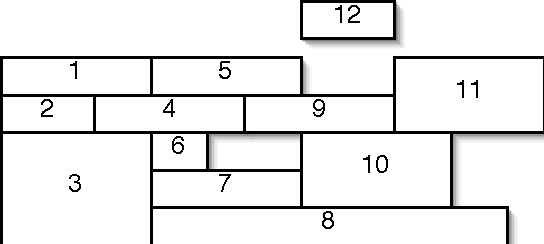
\includegraphics{job-grid}
    \end{itemize}
  \end{itemize}
\end{frame}
\subsection{Scheduler Commands}
\begin{frame}{Understanding the Scheduler}
There are several commands that can give you insight into the scheduler's
decisions.
\begin{itemize}
\item \texttt{showq} --- shows the state of the queue at that moment in time,
showing the running jobs in order of soonest to finish to longest to finish; the
idle jobs in order of priority; and the blocked jobs in the order they were
submitted
\item \texttt{diagnose -p} --- shows the factors that go into computing the
priority for all of the idle jobs
\item \texttt{checkjob \textit{jobnumber}} --- for idle jobs this will show why
the job can't start
\item \texttt{showstart \textit{jobnumber}} --- this makes a (poor) estimate of
when the job will start
\end{itemize}
\end{frame}
\section{Summary}
\subsection{Resources and Access}
\begin{frame}{Summary}
 \begin{itemize}
  \item Resources
   \begin{itemize}
    \item Lots of CPUs
    \item A reasonable amount of software
    \item Watch or subscribe to \url{http://cac.engin.umich.edu} for updates
   \end{itemize}
   \item Access
    \begin{itemize}
     \item All access is via the SSH family of commands: \texttt{ssh},
\texttt{sftp}, \texttt{scp}
     \item There are lots of clients for these commands for the different
platforms
     \item There is no graphical access, everything is via the command line
    \end{itemize}
 \end{itemize}
\end{frame}
\subsection{Job Management}
\begin{frame}{Summary}
 \begin{itemize}
   \item Job Submission
     \begin{itemize}
     \item Every job needs a PBS script file
     \item Two most important commands: \texttt{qsub} and \texttt{qstat -au \textit{uniqname}}
     \end{itemize}
   \item Job Scheduling
     \begin{itemize}
     \item Scheduling depends on a lot of factors, it is best to submit jobs and let the
scheduler optimize for their start.
     \end{itemize}
 \end{itemize}
\end{frame}
\subsection{Contact}
\begin{frame}{Summary}
 \begin{itemize}
 \item News: \url{http://cac.engin.umich.edu}
   \begin{itemize}
    \item RSS feed
    \item New of changes, outages, other pertinent piece of information
   \end{itemize}
  \item Contact: \url{cac-support@umich.edu}
   \begin{itemize}
    \item Questions or concerns should be sent here (not to an individual) since
this is read by six people.  The odds of a quick reply are best this way.
    \item We aren't parallel programmers, but we'll do what we can to help.
   \end{itemize}
 \end{itemize}
\end{frame}
\begin{frame}{Example}
 \alert{Change example to}
 \begin{block}{example}
  Open a shell....
  \begin{enumerate}
   \item<1>  \texttt{cp -r \textasciitilde brockp/mcnp\_example ~/}
   \item<2>  \texttt{cat mcnp.q}
   \item<3>  \texttt{module load mcnp5}
   \item<4>  \texttt{qsub mcnp.q}
   \item<5>  \texttt{qstat -u \$USER}
  \end{enumerate}
 \end{block}
\end{frame}
\end{document}
